\begin{figure}[h]
    \center
    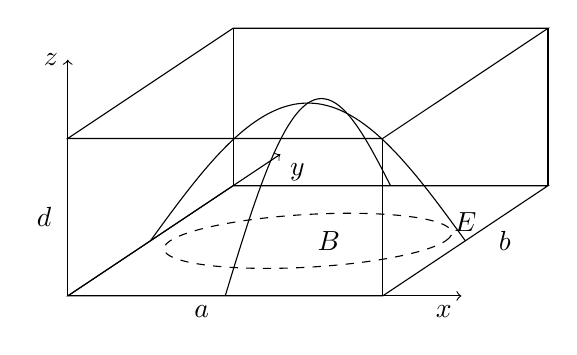
\begin{tikzpicture}[ % FISSA IL RIFERIMENTO IN MODO CORRETTO, ALTRIMENTRI --> (X,Z,Y)
        x={(1cm,0cm)},
        y={(0.6cm,0.4cm)},
        z={(0cm,1cm)}
        ]
            % Parametri
        \def\a{4}
        \def\b{3.5}
        \def\d{2}

        % Assi cartesiani
        \draw[->] (0,0,0) -- ({\a + 1},0,0) node[below left] {$x$};
        \draw[->] (0,0,0) -- (0,{\b + 1},0) node[below right] {$y$}; % below/above
        \draw[->] (0,0,0) -- (0,0,{\d + 1}) node[left] {$z$};

        % Vertici del parallelepipedo
        \coordinate (O) at (0,0,0);
        \coordinate (A) at (\a,0,0);
        \coordinate (B) at (\a,\b,0);
        \coordinate (C) at (0,\b,0);

        \coordinate (O1) at (0,0,\d);
        \coordinate (A1) at (\a,0,\d);
        \coordinate (B1) at (\a,\b,\d);
        \coordinate (C1) at (0,\b,\d);

        % Spigoli base
        \draw (O) -- (A) -- (B) -- (C) -- cycle;

        % Spigoli verticali
        \draw (O) -- (O1);
        \draw (A) -- (A1);
        \draw (B) -- (B1);
        \draw (C) -- (C1);

        % Spigoli superiori
        \draw (O1) -- (A1) -- (B1) -- (C1) -- cycle;

        % Etichette dimensioni
        \node at (\a/2, -0.5, 0) {$a$};
        \node at (\a+0.5, \b/2, 0) {$b$};
        \node at (-0.3, 0, \d/2) {$d$};

        % Centro della base
        \coordinate (M) at ({\a/2},{\b/2},0);

        % Ellisse sul piano xy centrata in M
        \draw[dashed] (M) ellipse [x radius={\a * 7/16 }, y radius={\b/4}] node[right] {$B$};

        % Funzione seno sul piano xy: z = 0, y = b/2
        \draw[domain=0:\a, smooth, variable=\x]
            plot ({\x},{\b/2},{ \d * 7/8 *sin(180/\a*\x)}) node[above] {$E$};
        
        \draw[domain=0:\b, smooth, variable=\y]
            plot ({\a/2},\y,{ \d * 7/8 *sin(180/\b *\y)});

    \end{tikzpicture}
    \caption{Campi all'interno della cavità}
    \label{figure:_cavità_parallelepipedo_campi}
\end{figure}